\documentclass[twoside,twocolumn,9pt,a4paper]{IEEEtran}
\usepackage{graphics,epsfig,amsmath,graphpap}
\usepackage{multirow,cite,hyperref}
%\usepackage[applemac]{inputenc}
\usepackage[utf8]{inputenc}
\usepackage[english]{babel}
\graphicspath{ {./Images/} } % Denna lade jag till som referar så man kan använd folder "Images"
\usepackage{float}
\usepackage{placeins}
\usepackage{placeins}
\raggedbottom

\begin{document}

\title{Parameter analysis in thermoacoustic mixing}
\author{
Ossian Eriksson (BME21), Jonathan Olsson (BME21)
\thanks{Handed in \today}
\thanks{Email adress:\{os7673er-s@student.lu.se, jo3405ol@student.lu.se\}}
\thanks{Project supervisor: Enrico Corato, LTH}
\thanks{Parameteranalys inom termoakustisk mixning} % ???????????????????????????
}
\maketitle

%-----------------------------------------------------------------------------------------------------------------------

\begin{abstract}
Text
\end{abstract}

%-----------------------------------------------------------------------------------------------------------------------

\section{Introduction} \label{secIntroduction}

Text \cite{Ward}.

\subsection{Background}

Text \cite{Bruus}:

\subsection{Thesis}

\section{Method} \label{secAfibMethods}

\subsection{General experimental setup}

Text

\begin{figure}[h]
\begin{center}
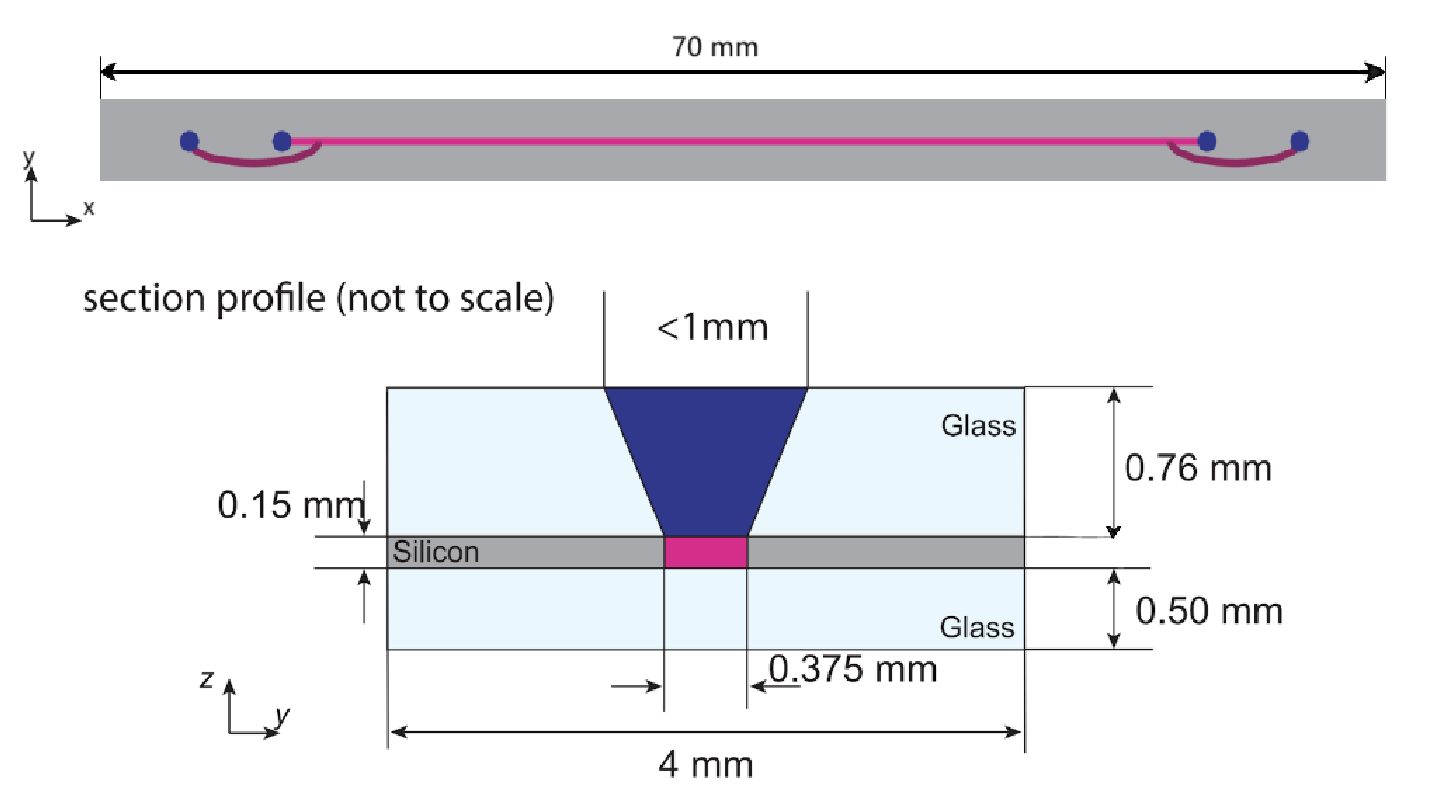
\includegraphics[width=7.5cm]{Images/Updated_figure1.png} %figurer sparas lämpligen i eps format
\caption{Dimensions of the microchip and of the cross section where the light blue is glass, gray is the silicon chip and the dark blue is the inlet of the channel and magenta is the channel itself. }
\label{DimensionMicrochip}
\end{center}
\end{figure} % Micro chip dimensions 1

\newpage
\begin{thebibliography}{99} % IEEE-format

\bibitem{Bruus} Bruus, H. (1997) ‘Basic concepts in Microfluidics’, \textit{Theoretical Microfluidics}, pp. 1–18.

\end{thebibliography}

\end{document}